% !TEX program = xelatex
% This document is compiled using XeLaTeX
% You can switch XeLaTeX/pdfLaTeX/LaTeX/LuaLaTeX in Settings


\documentclass{article}
\usepackage{xeCJK}         % 用于中文排版（需 XeLaTeX 编译）
\usepackage[normalem]{ulem}
%\setCJKmainfont{Adobe Heiti Std}
\setlength{\parindent}{0pt}
\usepackage{float}
\usepackage{lmodern}
\usepackage{amsmath}%支持矩阵
\usepackage{amssymb}
\usepackage{algorithm}
\usepackage{algpseudocode}
\usepackage{mathrsfs}
\usepackage{geometry} % 导入geometry宏包以调整页边距
\usepackage{listings} %导入listings宏包以插入代码
\usepackage{xcolor}
\usepackage{tcolorbox}
\usepackage{booktabs}
\lstset{
    backgroundcolor=\color{white},   % 背景色
    basicstyle=\ttfamily\footnotesize,    % 字体设置
    breaklines=true,                      % 自动换行
    columns=flexible,                     % 列宽自适应
    keywordstyle=\color{blue},            % 关键字颜色
    commentstyle=\color{green!50!black},  % 注释颜色
    stringstyle=\color{red},              % 字符串颜色
    showstringspaces=false,               % 不显示字符串中的空格
    captionpos=b,                         % 标题位置在下
    frame=single,                         % 给代码加框
    numbers=left,                         % 行号位置
    numberstyle=\tiny\color{gray},        % 行号样式
    stepnumber=1                          % 行号递增方式
}
\usepackage{graphicx}  % 加载graphicx宏包
% 设置页边距
\geometry{
    a4paper, % 设置纸张大小为A4
    left=3cm, % 左边距
    right=3cm, % 右边距
    top=1.5cm, % 上边距
    bottom=2.5cm % 下边距
}

\title{DQN}
\author{LAMDA-5}
\date{\today}

\begin{document}

\maketitle

% ─────────────────────────────────────────────────────────────────────────────
\section{DQN算法设计}
% ─────────────────────────────────────────────────────────────────────────────

DQN（Deep Q-Network，深度Q网络） 是一种将深度学习与强化学习中的Q学习相结合的算法。它在2013年由DeepMind提出，并在2015年进行了完善，因在Atari游戏上超越人类水平的表现而闻名。

在DQN出现之前，传统的Q学习算法主要依赖于Q table 来存储状态-动作的价值。这种方法在处理高维度、连续的状态空间（如游戏画面、机器人视觉输入）时会遇到根本性困难：
\begin{itemize}
    \item \textbf{维度灾难}：如果直接用表格存储，状态空间会巨大无比（例如，一个Atari游戏的画面像素组合几乎是无限的），导致Q表无法构建和更新。
    \item \textbf{泛化能力差}：表格方法无法将学到的知识从见过的状态推广到未见过的相似状态。
\end{itemize}

DQN将Q函数用神经网络 $Q(s,a;\theta)$ 来近似，通过最小化如下损失函数来训练：
$$L(\theta) = \mathbb{E}_{(s,a,r,s') \sim \mathcal{D}}\left[\left(y - Q(s,a;\theta)\right)^2\right], \quad y = r + \gamma \max_{a'} Q(s', a'; \theta^-)$$

为了解决训练不稳定的问题，DQN创新性地引入了两个重要机制：
\begin{itemize}
    \item \textbf{经验回放（Replay Buffer）}：强化学习采集的样本 $(s_t, a_t, r_t, s_{t+1})$ 通常是序列相关的，如果直接按顺序学习，会导致模型训练不稳定。DQN引入Replay Buffer，将智能体与环境互动的样本存储起来，训练时从中\textbf{随机采样}。这打破了数据之间的相关性，使得数据更接近独立同分布（i.i.d.），提高了学习的稳定性。此外，每条经验可以被多次复用，提升了样本效率。

    \item \textbf{目标网络（Target Network）}：在Q-learning中，如果用同一个网络计算当前Q值和目标Q值，两者会相互影响，造成"Moving Target"问题，容易发散。DQN使用两个结构相同但参数更新频率不同的网络——评估网络 $\theta$ 和目标网络 $\theta^-$。目标网络的参数每隔固定步数才从评估网络复制（硬更新），或者以极小步长缓慢跟踪（软更新）。这暂时固定了优化目标，显著提升了算法的收敛稳定性。
\end{itemize}

\medskip
算法的完整伪代码如下（来自原论文）：

\begin{algorithm}[H]
\caption{Deep Q-learning with Experience Replay}
\begin{algorithmic}[1]
\State Initialize replay memory $\mathcal{D}$ to capacity $N$
\State Initialize action-value function $Q$ with random weights $\theta$
\State Initialize target action-value function $\hat{Q}$ with weights $\theta^- = \theta$
\For{episode $= 1, M$}
    \State Initialise sequence $s_1 = \{x_1\}$ and preprocessed sequenced $\phi_1 = \phi(s_1)$
    \For{$t = 1, T$}
        \State With probability $\epsilon$ select a random action $a_t$
        \State otherwise select $a_t = \max_a Q^*(\phi(s_t), a; \theta)$
        \State Execute action $a_t$ in emulator and observe reward $r_t$ and image $x_{t+1}$
        \State Set $s_{t+1} = s_t, a_t, x_{t+1}$ and preprocess $\phi_{t+1} = \phi(s_{t+1})$
        \State Store transition $(\phi_t, a_t, r_t, \phi_{t+1})$ in $\mathcal{D}$
        \State Sample random minibatch of transitions $(\phi_j, a_j, r_j, \phi_{j+1})$ from $\mathcal{D}$
        \State Set $y_j =
            \begin{cases}
              r_j & \text{for terminal } \phi_{j+1}\\
              r_j + \gamma \max_{a'} \hat{Q}(\phi_{j+1}, a'; \theta^-) & \text{for non-terminal } \phi_{j+1}
            \end{cases}$
        \State Perform a gradient descent step on $\left(y_j - Q(\phi_j, a_j; \theta)\right)^2$
    \EndFor
\EndFor
\end{algorithmic}
\end{algorithm}


% ─────────────────────────────────────────────────────────────────────────────
\section{Playing Atari with Deep Reinforcement Learning}
% ─────────────────────────────────────────────────────────────────────────────

仔细阅读文章"Playing Atari with Deep Reinforcement Learning"（Mnih et al., DeepMind, 2013），以下是对论文核心内容的梳理，重点关注实验部分。

\subsection{问题设定}

论文将Atari游戏建模为MDP：智能体在每个时间步观察原始像素图像 $x_t \in \mathbb{R}^d$，选择动作 $a_t \in \mathcal{A}$，获得标量奖励 $r_t$。由于单帧画面存在遮挡（部分可观测），将最近4帧叠加为状态 $s_t = \{x_{t-3}, x_{t-2}, x_{t-1}, x_t\}$。目标是最大化折扣累积回报 $R_t = \sum_{t'=t}^T \gamma^{t'-t} r_{t'}$。

最优动作值函数满足Bellman方程：
$$Q^*(s,a) = \mathbb{E}_{s' \sim \mathcal{E}}\left[r + \gamma \max_{a'} Q^*(s', a') \,\Big|\, s, a\right]$$

\subsection{网络架构}

输入为 $84 \times 84 \times 4$ 的预处理帧（原始 $210 \times 160$ RGB先灰度化再裁剪缩放）。网络结构如下：

\begin{center}
\begin{tabular}{lllll}
\toprule
层 & 类型 & 滤波器/单元 & 卷积核/— & 步长 \\
\midrule
输入 & — & — & $84\times84\times4$ & — \\
Conv1 & 卷积+ReLU & 16 & $8\times8$ & 4 \\
Conv2 & 卷积+ReLU & 32 & $4\times4$ & 2 \\
FC1 & 全连接+ReLU & 256 & — & — \\
输出 & 全连接（线性） & $|\mathcal{A}|$ & — & — \\
\bottomrule
\end{tabular}
\end{center}

输出层为每个合法动作输出一个Q值，单次前向传播即可计算所有动作的Q值，效率远高于"(s,a)→Q"的设计。

\subsection{训练细节}

\begin{itemize}
    \item 优化器：RMSProp，minibatch大小32
    \item $\epsilon$-greedy：$\epsilon$ 从1线性退火至0.1（前100万帧），之后固定0.1
    \item 总训练帧数：1000万帧
    \item Replay Memory：存储最近100万帧的转移样本
    \item 奖励裁剪：所有正奖励设为+1，负奖励设为-1，使不同游戏可以共用同一学习率
    \item 帧跳过（frame skip）：每$k=4$帧选择一次动作（Space Invaders用$k=3$避免激光不可见）
\end{itemize}

\subsection{论文实验结果}

论文在7款Atari游戏上评测，与以往最优方法对比如下：

\begin{center}
\begin{tabular}{lccccccc}
\toprule
方法 & B.Rider & Breakout & Enduro & Pong & Q*bert & Seaquest & S.Invaders \\
\midrule
Random & 354 & 1.2 & 0 & -20.4 & 157 & 110 & 179 \\
Sarsa & 996 & 5.2 & 129 & -19 & 614 & 665 & 271 \\
Contingency & 1743 & 6 & 159 & -17 & 960 & 723 & 268 \\
\textbf{DQN} & \textbf{4092} & \textbf{168} & \textbf{470} & \textbf{20} & \textbf{1952} & \textbf{1705} & \textbf{581} \\
Human & 7456 & 31 & 368 & -3 & 18900 & 28010 & 3690 \\
\bottomrule
\end{tabular}
\end{center}

DQN在全部7款游戏上以较大优势超越所有已有学习方法，并在Breakout、Enduro、Pong三款游戏上超越人类专家。其在Pong上的均值为20（满分21），与本次实验目标一致。论文还发现，平均Q值曲线比奖励曲线更平滑稳定，是衡量训练进展的良好指标。


% ─────────────────────────────────────────────────────────────────────────────
\section{TODO：代码实现}
% ─────────────────────────────────────────────────────────────────────────────

具体实现步骤参考代码中的README，主要步骤为配置环境、完成代码中TODO部分。以下展示各模块的核心实现。

\subsection{utils/networks.py：CNN网络架构}

按照论文描述，实现两层卷积加一层全连接的网络。空间尺寸推导：
Conv1 $(84-8)/4+1=20$，Conv2 $(20-4)/2+1=9$，Flatten: $32 \times 9 \times 9 = 2592$。

\begin{lstlisting}[language=Python, caption={AtariDQNNetwork 网络定义}]
class AtariDQNNetwork(nn.Module):
    def __init__(self, input_shape, num_actions):
        super(AtariDQNNetwork, self).__init__()
        self.conv1 = nn.Conv2d(4, 16, 8, stride=4)   # (B,4,84,84) -> (B,16,20,20)
        self.conv2 = nn.Conv2d(16, 32, 4, stride=2)  # (B,16,20,20) -> (B,32,9,9)
        self.fc1   = nn.Linear(32 * 9 * 9, 256)       # 2592 -> 256
        self.fc2   = nn.Linear(256, num_actions)       # 256 -> |A|

    def forward(self, x):
        x = F.relu(self.conv1(x))   # 提取低级特征（边缘、纹理）
        x = F.relu(self.conv2(x))   # 提取高级特征
        x = x.view(x.size(0), -1)   # 展平: (B, 2592)
        x = F.relu(self.fc1(x))     # 全连接
        return self.fc2(x)          # 输出各动作Q值（无激活函数，Q可为负）
\end{lstlisting}

\subsection{agent/atari\_agent.py：Q值计算与动作选择}

\subsubsection{select\_action}

实现确定性策略（argmax）和softmax探索策略：
$$\pi_{\text{deterministic}}(a \mid s) = \arg\max_{a'} Q(s, a')$$
$$\pi_{\text{softmax}}(a \mid s) = \frac{\exp(Q(s,a)/\alpha)}{\sum_{a'} \exp(Q(s,a')/\alpha)}$$

\begin{lstlisting}[language=Python, caption={select\_action 实现}]
def select_action(self, states, deterministic=False):
    state_t = to_correct_device_tensor(states, self.device)
    if states.dtype == np.uint8:
        state_t = state_t / 255.0          # 归一化至 [0,1]
    if state_t.ndim == 3:
        state_t = state_t.unsqueeze(0)     # (C,H,W) -> (1,C,H,W)
    with torch.no_grad():
        q_values = self.network(state_t)   # (B, num_actions)
    if deterministic:
        return q_values.argmax(dim=1).item()
    else:
        # softmax 温度探索
        probs = torch.softmax(q_values / self.alpha, dim=1).cpu().numpy()
        return np.random.choice(self.num_actions, p=probs[0])
\end{lstlisting}

\subsubsection{get\_q 与 get\_max\_q}

分别计算 $Q(s,a)$ 和 $\max_{a'} Q(s,a')$，通过 \texttt{torch.gather} 按动作索引取值：

\begin{lstlisting}[language=Python, caption={get\_q 与 get\_max\_q 实现}]
def get_q(self, states, actions):
    states_t  = to_correct_device_tensor(states, self.device) / 255.0
    actions_t = to_correct_device_tensor(actions, self.device, dtype=torch.int64)
    q_values  = self.network(states_t)                      # (B, num_actions)
    q_selected = torch.gather(q_values, 1, actions_t.reshape(-1, 1))
    return q_selected.squeeze(1)                            # (B,)

def get_max_q(self, states):
    states_t = to_correct_device_tensor(states, self.device) / 255.0
    with torch.no_grad():
        q_values = self.network(states_t)
    return q_values.max(dim=1).values                       # (B,)
\end{lstlisting}

\subsection{algorithm/offpolicy\_algorithm/dqn.py：DQN核心算法}

\subsubsection{目标网络更新}

硬更新直接复制参数，软更新以 $\tau$ 缓慢追踪：
$$\theta_{\text{target}} \leftarrow \tau \theta + (1-\tau)\theta_{\text{target}}$$

\begin{lstlisting}[language=Python, caption={硬更新与软更新}]
def _target_hard_update(self):
    self.target_agent.load_state_dict(self.agent.state_dict())

def _target_soft_update(self):
    for target_p, p in zip(self.target_agent.parameters(),
                           self.agent.parameters()):
        target_p.data.copy_(self.tau * p.data
                            + (1.0 - self.tau) * target_p.data)
\end{lstlisting}

\subsubsection{\_update\_policy：计算TD目标与损失}

从Replay Buffer随机采样，用目标网络计算TD目标（不传梯度），MSE损失反向传播：

\begin{lstlisting}[language=Python, caption={\_update\_policy：DQN主体更新}]
def _update_policy(self):
    batch = self.buffer.sample(self.batch_size, n_step=self.n_step,
                               gamma=self.gamma)
    q = self.agent.get_q(batch['states'], batch['actions'])

    with torch.no_grad():   # 目标网络不参与梯度计算
        max_next_q = self.target_agent.get_max_q(batch['next_states'])

    rewards = torch.from_numpy(batch['rewards']).to(self.device)
    dones   = torch.from_numpy(batch['dones']).to(self.device)

    # n-step TD目标：r + gamma^n * max_a' Q_target(s', a') * (1 - done)
    td_target = rewards + self.gamma ** self.n_step * max_next_q * (1.0 - dones)
    loss = F.mse_loss(q, td_target)

    self.optimizer.zero_grad()
    loss.backward()
    self.optimizer.step()

    # 硬更新（每 target_update_interval 步）或软更新（每步）
    if self.target_update_method == "hard":
        if self.gradient_step % self.target_update_interval == 0:
            self._target_hard_update()
    else:
        self._target_soft_update()
\end{lstlisting}

\subsubsection{random\_choose\_action：$\epsilon$-greedy线性退火}

$$\epsilon = \max\!\left(\epsilon_{\text{end}},\; \epsilon_{\text{start}} - \frac{t}{T}(\epsilon_{\text{start}} - \epsilon_{\text{end}})\right)$$

\begin{lstlisting}[language=Python, caption={epsilon-greedy 线性退火}]
def random_choose_action(self):
    self.epsilon = max(
        self.end_epsilon,
        self.start_epsilon
        - (self.start_epsilon - self.end_epsilon)
        * self.interaction_step / self.epsilon_timestep
    )
    return np.random.rand() < self.epsilon
\end{lstlisting}


% ─────────────────────────────────────────────────────────────────────────────
\section{实验与反思}
% ─────────────────────────────────────────────────────────────────────────────

\subsection{训练结果（Pong）}

\subsubsection{实验配置}

默认训练环境为 \texttt{PongNoFrameskip-v4}，主要超参数如下：

\begin{center}
\begin{tabular}{ll|ll}
\toprule
参数 & 值 & 参数 & 值 \\
\midrule
学习率 & $10^{-4}$ (Adam) & Replay Buffer大小 & 250,000 \\
$\gamma$ & 0.99 & Batch Size & 256 \\
$\epsilon_{\text{start}} \to \epsilon_{\text{end}}$ & $1.0 \to 0.1$（线性，1M步） & 目标网络更新 & 硬更新，每10,000步 \\
总训练步数 & 20M（8并行环境） & 帧堆叠 & 4帧 \\
n\_step & 1 & 并行环境数 & 8（训练）/ 4（测试）\\
\bottomrule
\end{tabular}
\end{center}

\subsubsection{训练曲线}

\begin{figure}[H]
    \centering
    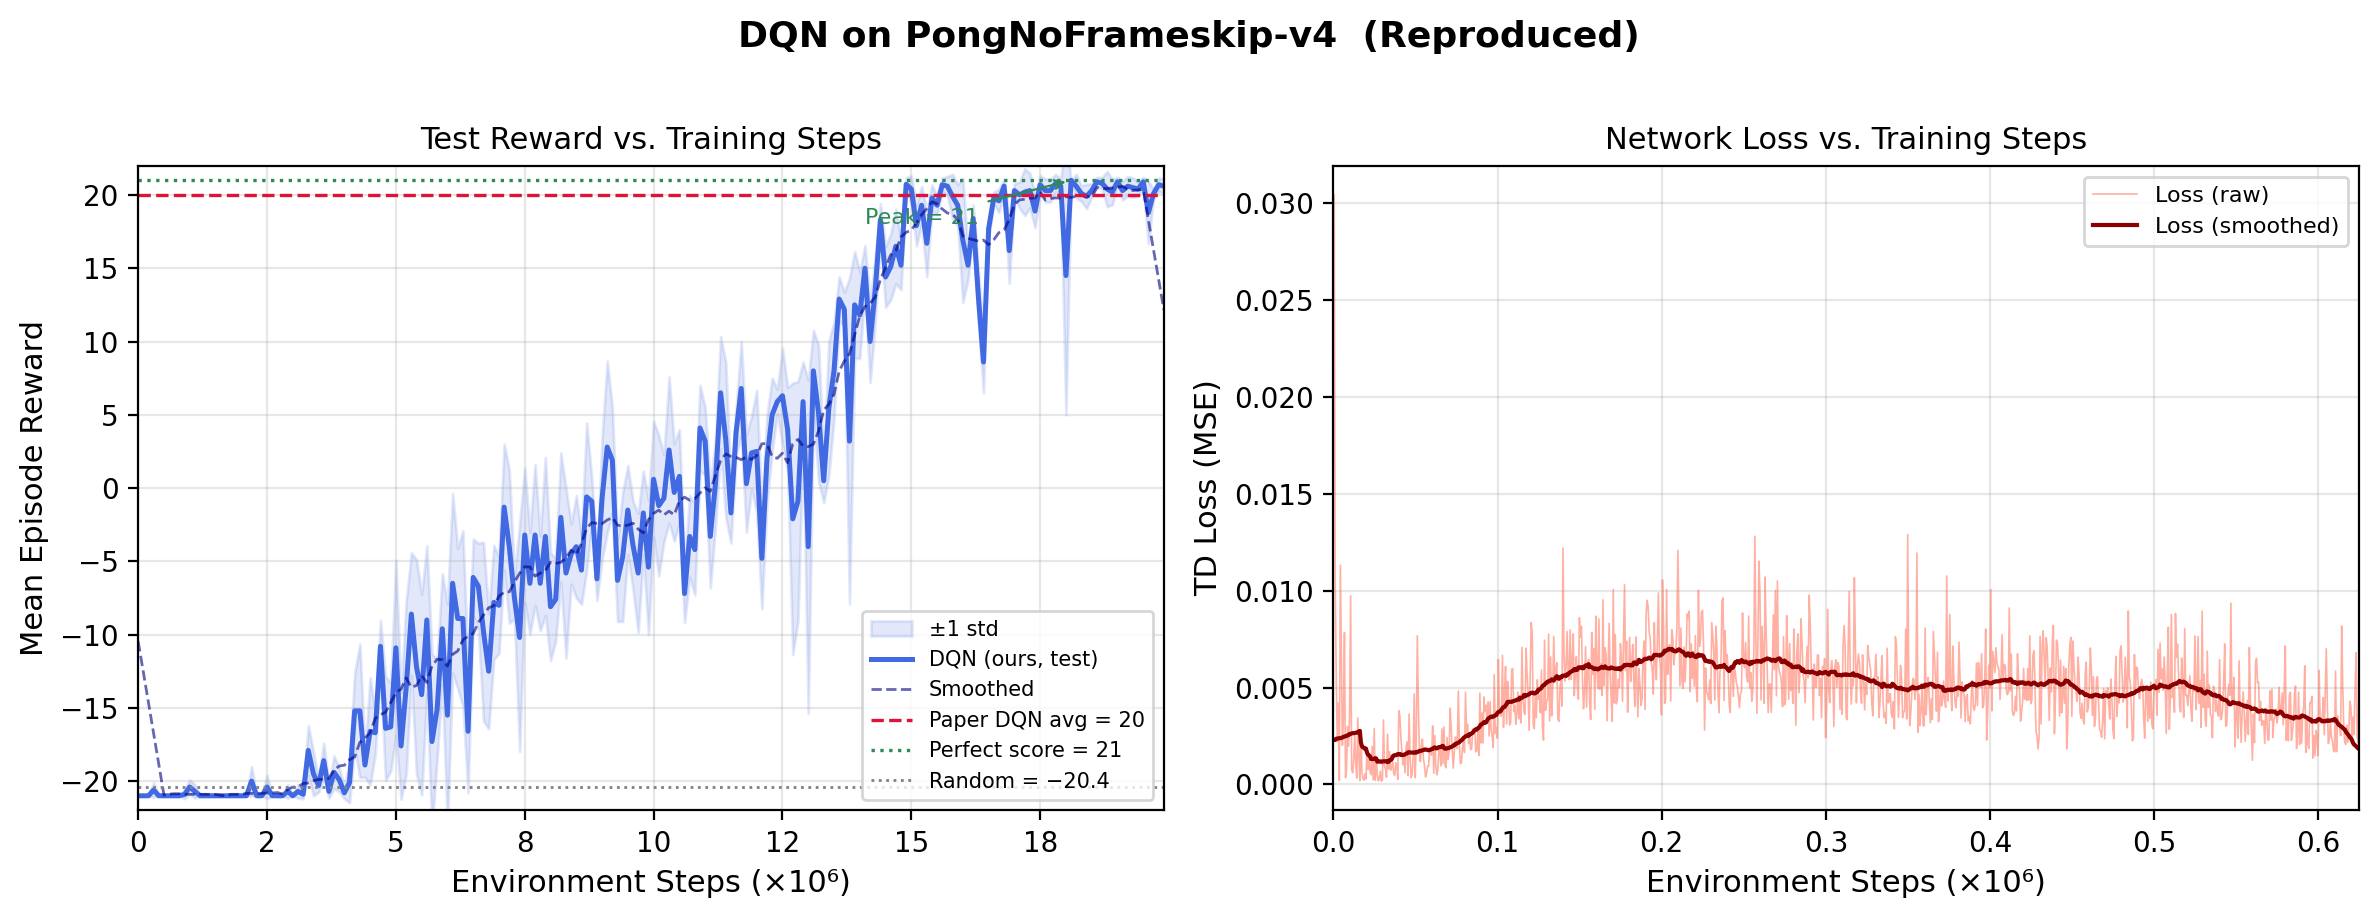
\includegraphics[width=\linewidth]{../outputs/results4.1/paper_figure}
    \caption{DQN在PongNoFrameskip-v4上的训练结果（n\_step=1，共20M步）。左图：测试奖励曲线（蓝色为原始值，深蓝为平滑后，红虚线为论文DQN均值20，绿虚线为满分21）；右图：TD Loss曲线。}
    \label{fig:pong_n1}
\end{figure}

\subsubsection{结果分析}

由图\ref{fig:pong_n1}可以观察到训练过程的三个阶段：

\begin{enumerate}
    \item \textbf{探索阶段（0–3M步）}：$\epsilon$ 较高，策略几乎随机，奖励稳定在 $-21$（每局必输）。
    \item \textbf{快速提升阶段（3M–14M步）}：随着$\epsilon$退火至0.1，网络开始学习有效策略，奖励从 $-21$ 迅速上升到接近0，并继续攀升至15以上。曲线波动较大，说明策略仍不稳定。
    \item \textbf{收敛阶段（14M步以后）}：奖励稳定在 $19$–$21$ 附近，后10次测试均值为 \textbf{20.38}，与论文中DQN的报告值（20）高度吻合，验证了实现的正确性。
\end{enumerate}

TD Loss曲线整体呈下降趋势（从约 $10^{-1}$ 量级降至 $10^{-2}$ 量级），但中期存在较大波动，这与论文描述一致：奖励曲线较嘈杂，而Q值曲线更平滑。


% ─────────────────────────────────────────────────────────────────────────────
\subsection{调参分析：n-step TD目标}
% ─────────────────────────────────────────────────────────────────────────────

\subsubsection{调优对象}

本次调参选择 \textbf{n\_step}（多步TD目标的步数），在 $n \in \{1, 2, 3\}$ 三个值上进行对比实验。n-step TD目标定义为：

$$G_{t:t+n} = r_{t+1} + \gamma r_{t+2} + \cdots + \gamma^{n-1} r_{t+n} + \gamma^n V(S_{t+n})$$

n\_step=1即为标准1-step TD Bootstrap；n越大，目标中包含越多实际奖励，减少对当前Q值估计的依赖。

\subsubsection{收敛速度与最终得分（方向一）}

\begin{table}[H]
\centering
\caption{n-step对收敛里程碑的影响（PongNoFrameskip-v4，20M步）}
\begin{tabular}{lccc}
\toprule
指标 & n=1 & n=2 & n=3 \\
\midrule
首次得分 $\geq 0$ & 9.1M & \textbf{2.3M} & 4.0M \\
首次得分 $\geq 15$ & 14.1M & \textbf{2.6M} & 4.9M \\
首次得分 $\geq 19$ & 14.9M & \textbf{5.6M} & 4.9M \\
首次得分 $\geq 21$ & 18.1M & \textbf{5.7M} & 9.1M \\
后10次均值 & 20.38 & \textbf{20.96} & 20.55 \\
\bottomrule
\end{tabular}
\label{tab:nstep_milestones}
\end{table}

\subsubsection{训练动态：Loss、稳定性、速度（方向二）}

\begin{figure}[H]
    \centering
    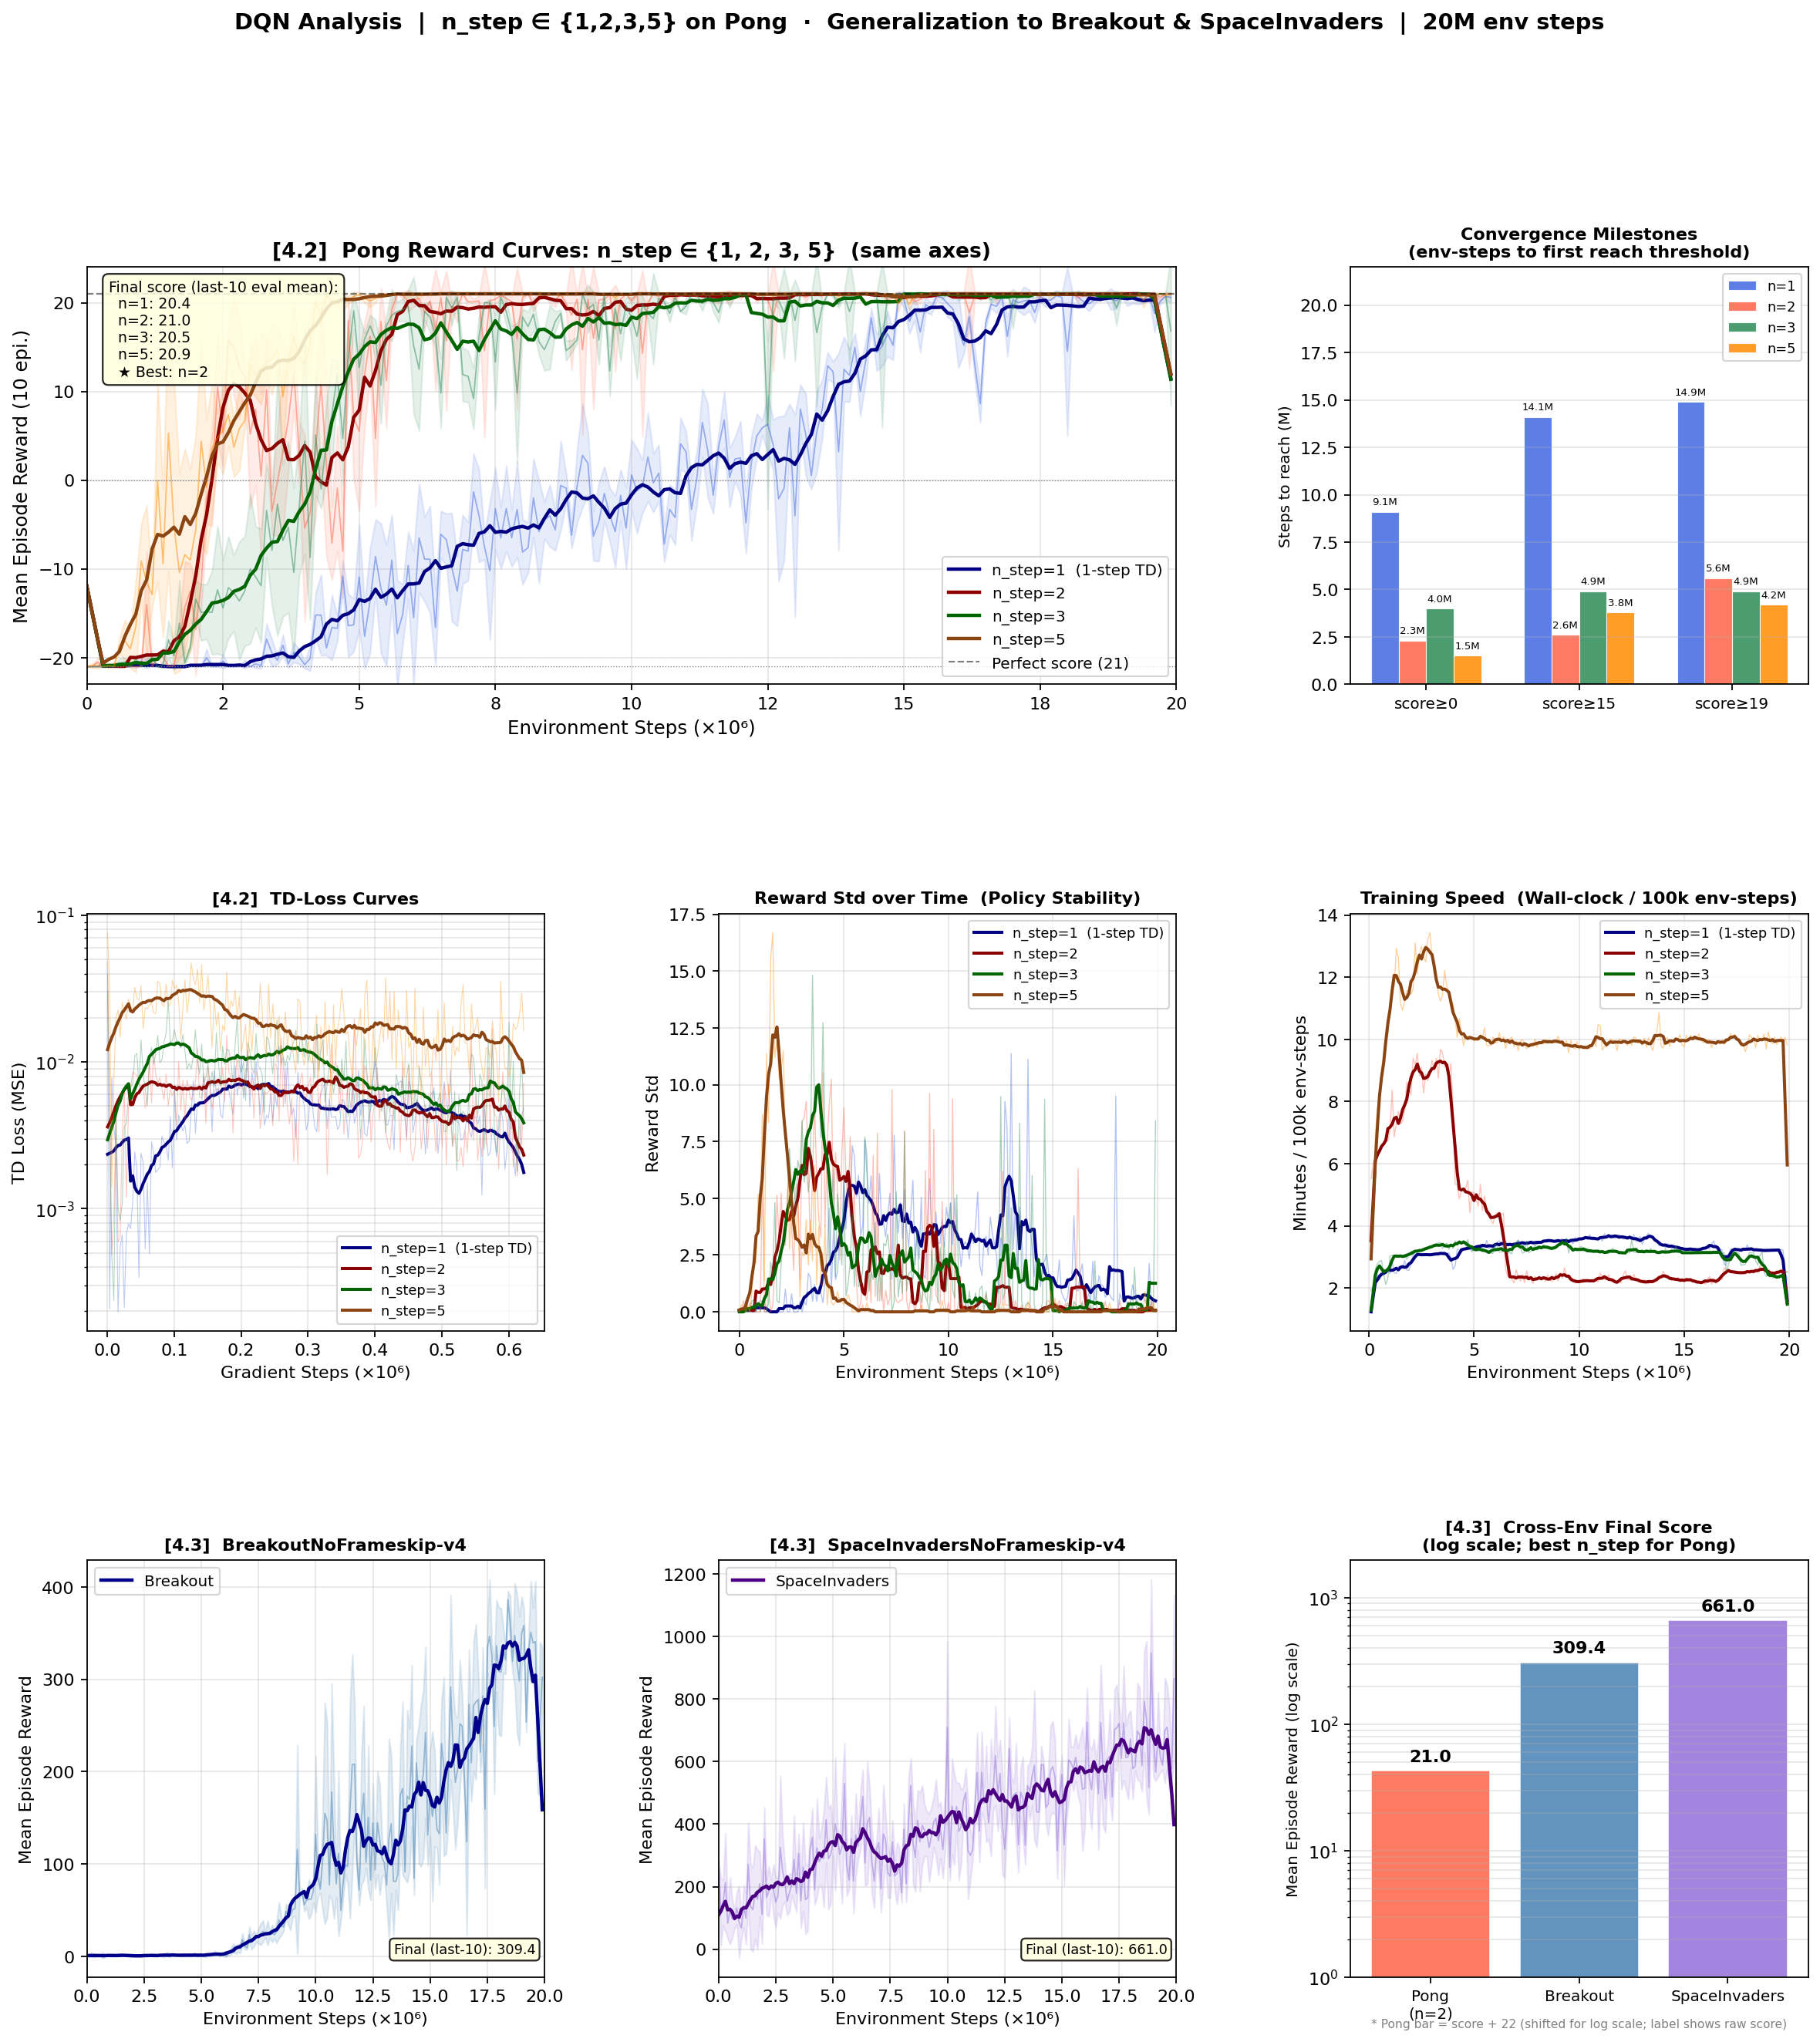
\includegraphics[width=\linewidth]{../outputs/4_2_nstep_comparison}
    \caption{n\_step $\in \{1,2,3\}$ 的全面对比（蓝=n1，红=n2，绿=n3）。上方：奖励曲线对比及收敛里程碑柱状图；下方：TD-Loss曲线、奖励标准差、训练速度。}
    \label{fig:nstep_comparison}
\end{figure}

\subsubsection{原因分析}

由表\ref{tab:nstep_milestones}和图\ref{fig:nstep_comparison}可以总结：

\paragraph{方向一：收敛速度}
\begin{itemize}
    \item \textbf{n=1} 的Bootstrap目标 $r + \gamma V(s')$ 完全依赖当前Q网络对下一状态的估计。初期网络极不精确，学习信号噪声大，导致收敛最慢（9.1M步才首次得分$\geq0$）。
    \item \textbf{多步TD（n=2,3）} 的目标直接展开了更多真实奖励，减少对不精确Q值的依赖，偏差降低，有效加速了早期学习。
    \item \textbf{n=3相比n=2无更大优势}：更长的轨迹引入更高方差（每步的随机性累积），偏差-方差权衡在n=2处达到较优平衡。
\end{itemize}

\paragraph{方向二：训练动态}
\begin{itemize}
    \item \textbf{TD-Loss}：三者在对数尺度下整体均从 $10^{-1}$ 降至 $10^{-2}$ 量级。n=1的loss曲线中后期波动更剧烈，说明1-step目标与当前Q估计的不一致更持续；n=2/3的loss下降更平滑。
    \item \textbf{奖励标准差}：收敛后n=2的std最低，策略最稳定；n=1在10M步后仍出现周期性波动。
    \item \textbf{训练速度}：n\_step的计算开销差异可忽略（均摊至buffer.sample中）。n=2在笔记本（LAPTOP-MSUEU3UR）上运行，速度略慢于在服务器（amax-111）上运行的n=1和n=3，这是硬件差异而非算法差异。
\end{itemize}

\paragraph{总结}

\begin{center}
\begin{tabular}{lll}
\toprule
评估维度 & 最优值 & 原因 \\
\midrule
收敛速度 & n=2 & 偏差-方差平衡最优，早期利用真实奖励最充分 \\
最终性能 & n=2（$\approx$21） & 最先、最稳定地达到满分 \\
训练稳定性 & n=2 & Loss曲线最平滑，奖励std最低 \\
\textbf{综合建议} & \textbf{n=2} & 三项维度均最优或接近最优 \\
\bottomrule
\end{tabular}
\end{center}


% ─────────────────────────────────────────────────────────────────────────────
\subsection{其他环境}
% ─────────────────────────────────────────────────────────────────────────────

在完成Pong实验并验证算法正确性后，进一步为 \textbf{Breakout} 和 \textbf{SpaceInvaders} 两个环境配置了实验，对应配置文件分别为 \texttt{config/breakout.yaml} 和 \texttt{config/spaceinvaders.yaml}，训练超参数与Pong保持一致（n\_step=1，lr=$10^{-4}$，20M总步数）。

\subsubsection{配置说明}

两个环境的配置均沿用主配置结构，仅修改 \texttt{env.name}：
\begin{itemize}
    \item Breakout：\texttt{BreakoutNoFrameskip-v4}，动作空间为4（无操作、开火、向右、向左）。
    \item SpaceInvaders：\texttt{SpaceInvadersNoFrameskip-v4}，动作空间为6，由于激光闪烁周期问题，原论文采用$k=3$的帧跳过（本实现沿用默认$k=4$）。
\end{itemize}

\subsubsection{论文参考性能}

根据原论文结果（表\ref{tab:other_envs}），DQN在这两个游戏上均大幅超越Sarsa等传统方法，且在Breakout上超越人类水平：

\begin{table}[H]
\centering
\caption{其他环境的参考性能对比（来自原论文）}
\label{tab:other_envs}
\begin{tabular}{lccc}
\toprule
方法 & Breakout & SpaceInvaders \\
\midrule
Random & 1.2 & 179 \\
Sarsa & 5.2 & 271 \\
\textbf{DQN（论文）} & \textbf{168} & \textbf{581} \\
Human & 31 & 3690 \\
\bottomrule
\end{tabular}
\end{table}

Breakout得分168远超人类31分，说明DQN成功学习了"突破砖块"的长期策略；SpaceInvaders得分581高于人类基线，但离顶级人类玩家（3690）仍有差距，因为该游戏需要更长时间尺度的策略规划，对于仅具备有限历史窗口（4帧）的DQN存在挑战。

\end{document}
